% Free range VHDL
% Authors: Bryan Mealy, Fabrizio Tappero
% Date: November, 2011
%
% (C) 2011 B. Mealy, F. Tappero
%
% !TEX root = master.tex
%
\chapter{Structural Modeling In VHDL}
As was mentioned earlier, there are generally three approaches to writing VHDL code: data-flow modeling, behavioral modeling and structural modeling.

Up to this point, this book has only dealt with data-flow and behavioral models. This section presents an introduction to structural modeling. 

As digital designs become more complex, it becomes less likely that any one design can be implemented with any one of the three types of VHDL models. We have already seen this property in dealings with FSMs where we mixed process statements (behavioral modeling) with selective signal assignment statements (data-flow modeling). The result was a hybrid VHDL model. By its very nature, structural modeling is likewise a hybrid VHDL model. Most complex designs could be considered structural models, i.e. if they are implemented using sound coding procedures. 

The design of complex digital circuits using VHDL should closely resemble the structure of complex computer programs. Many of the techniques and practices used to construct large and well structured computer programs written in higher-level languages should also be applied when using VHDL. This common structure we are referring to is the ever so popular modular approach to coding. The term structural modeling is the terminology that VHDL uses for the modular design. The VHDL modular design approach directly supports hierarchical design which is essentially employed when attempting to understand complex digital designs. 

The benefits of modular design to VHDL are similar to the benefits that modular design or object-oriented design provides for higher-level computer languages. Modular designs promote understandability by packing low-level functionality into modules. These modules can be easily reused in other designs thus saving the designer time by removing the need to reinvent and re-test the wheel. The hierarchical approach extends beyond code written on file level. VHDL modules can be placed in appropriately named files and libraries in the same way as higher-level languages. Moreover, there are often libraries out there that contain useful modules that can only be accessed using a structural-modeling approach. Having access to these libraries and being fluent in their use will serve to increase your perception as a VHDL guru.

After all the commentary regarding complex designs, we present a few simple examples. Though the structural approach is most appropriately used in complex digital designs, the examples presented in this section are rather simplistic in nature. These examples show the essential details of VHDL structural modeling. It is up to the designer to conjure up digital designs where a structural modeling approach would be more appropriate. Keep in mind that your first exposure to structural modeling may be somewhat rough. Although there is some new syntax to become familiar with, once you complete a few structural designs, this new syntax becomes ingrained in your brain and it becomes second nature to apply where required.

The tendency at this juncture in your VHDL programming career is to use some type of schematic capture software instead of learning the structural modeling approach. The fact is that no one of consequence uses the schematic capture software except for tired old university professors who are more interested in selling books than they are in teaching modern approach to VHDL modeling. The funny part about this entire process is that the schematic capture software is a tool that allows you to visually represent circuits but in the end generates VHDL code (the only thing the synthesizer understands is VHDL code).

\section{VHDL Modularity with Components}
The main tool for modularity in higher-level languages such as C is the function. In other computer languages, similar modularity is accomplished through the use of methods, procedures and subroutines. The approach used in C is to 1) name the function interface you plan on writing (the function declaration), 2) code what the function will do (the function body), 3) let the program know it exists and is available to be called (the prototype) and 4) call the function from the main portion of the code. In VDHL modularity is achieved via the use of \textbf{packages}, \textbf{components} and \textbf{functions}. In the following sections we are going to see how to use \texttt{components}.

The approach to use a \texttt{component} in VHDL  is: 1) name the module you plan to describe (the entity), 2) describe what the module will do (the architecture), 3) let the program know the module exists and can be used (component declaration) and 4) use the module in your code (component instantiation, or mapping). The similarities between these two approaches are listed in Table \ref{vhdl_c_comp}.

\begin{table}[!b]
\centering
\footnotesize\textsf{\begin{tabular}{ l l }
\hline
\rowcolor{gray} \textbf{C programming language} & \textbf{VHDL}\\
\hline
\rowcolor{light-gray} Describe function interface & The entity\\
\hline
Describe what the function does (coding) & The architecture \\
\hline
\rowcolor{light-gray} Provide a function prototype to main program & Component declaration \\
\hline
Call the function from main program & Component instantiation or mapping \\
\hline
\end{tabular}}
\caption{Similarities between modules in C and VHDL.}
\label{vhdl_c_comp}
\end{table}

Let us now use these principles in a practical example. Our approach is to describe a template-type approach to VHDL structural design using a simple and well-known combinational circuit.

\begin{leftbar}
\begin{minipage}[t]{0.52\textwidth}
\vspace{10pt}
\noindent
\textbf{EXAMPLE 22.}
Design a 3-bit comparator using a VHDL structural modeling. The interface to this circuit is described in the diagram below.
\end{minipage}
\begin{minipage}[t]{0.47\textwidth}
\vspace{0pt}\raggedright
    \centering
	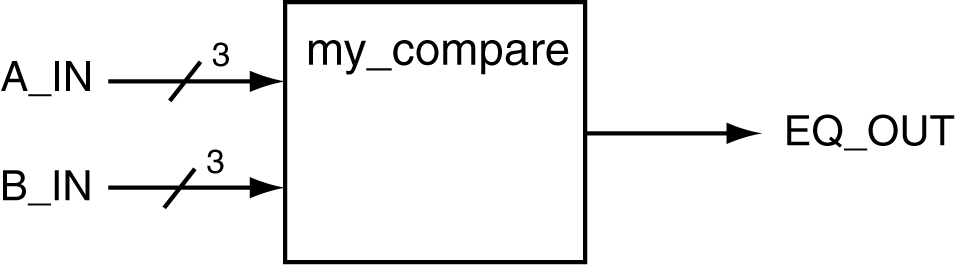
\includegraphics[width=5.2cm]{smu_vhdl/ex22.png}
\end{minipage}
\end{leftbar}

\noindent
\textbf{SOLUTION.} A comparator is one of the classic combinatorial circuits that every digital design engineer must derive at some point in his career. The solution presented here implements the discrete gate version of the circuit which is shown in Fig.~\ref{ex22_comp}. Once again, the solution presented here is primarily an example of a VHDL structural model and does not represent the most efficient method to represent a comparator using VHDL. 

The approach of this solution is to model each of the discrete gates as individual blocks. In this case, they are actually simple gates but the interfacing requirements of the VHDL structural approach are the same regardless of whether the circuit elements are simple gates or complex digital subsystems.

The circuit shown in Fig.~\ref{ex22_comp} contains some extra information that relates to its VHDL structural implementation. First, the dashed line represents the boundary of the top-level VHDL entity; therefore signals that cross this boundary must appear in the entity declaration for this implementation. Second, each of the internal signals is given a name. In this case, internal signals are defined to be signals that do not cross the dashed entity boundary. This is a requirement for VHDL structural implementations as these signals must be assigned to the various sub-modules in the interior of the design (somewhere in the architecture). 

\begin{figure}[!h]
    \centering
	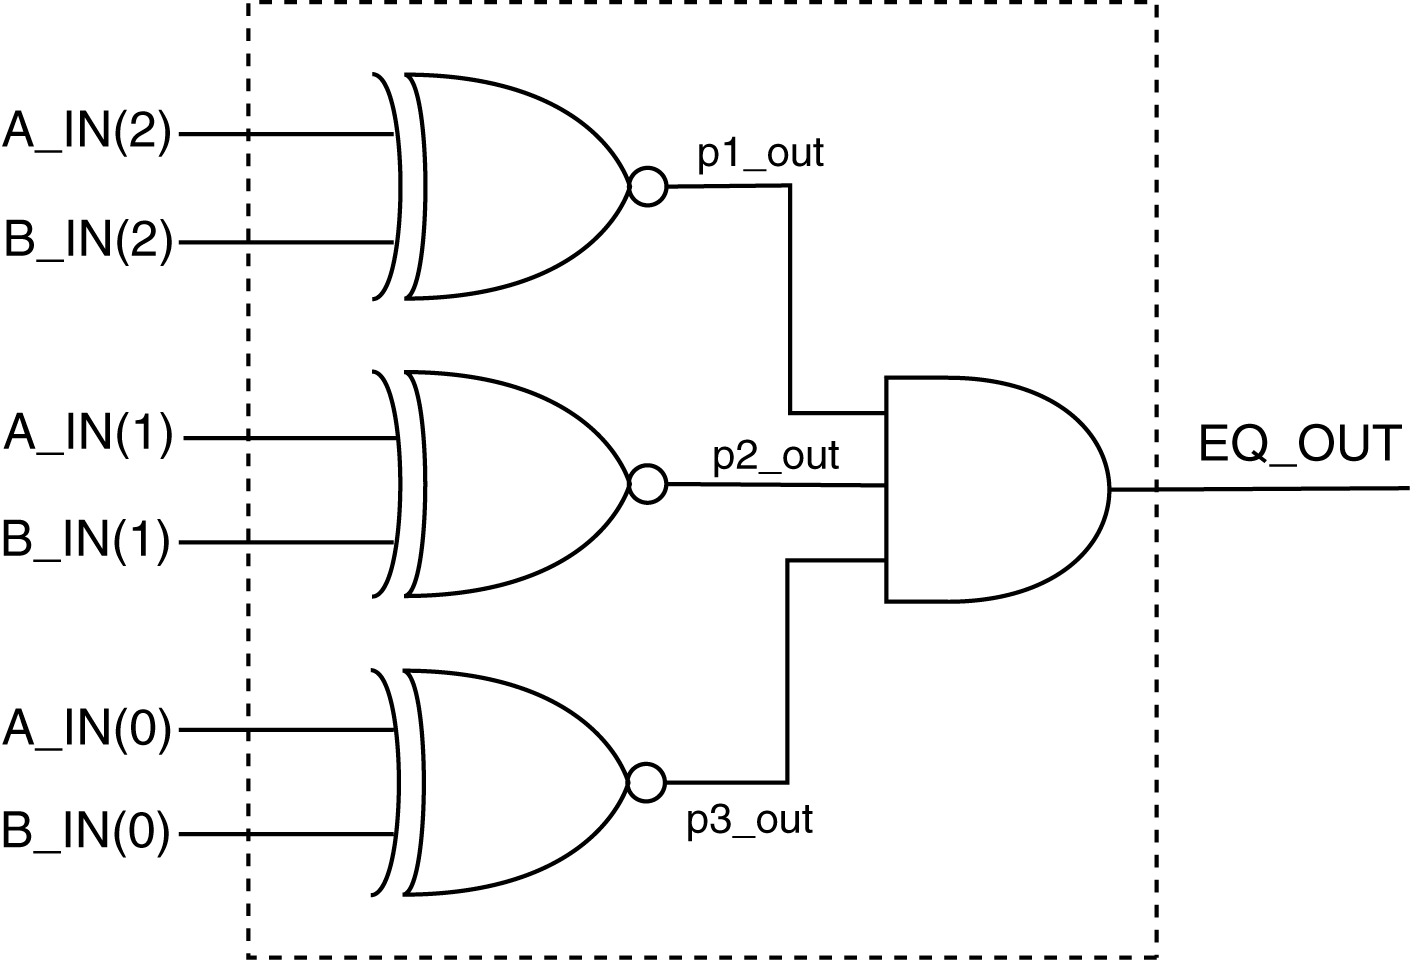
\includegraphics[width=7cm]{smu_vhdl/ex22_comp.png}
	\caption{Discrete gate implementation of a 3-bit comparator.}
	\label{ex22_comp}
\end{figure}

The first part of the solution is to provide entity and architecture implementations for the individual gates shown in Fig.~\ref{ex22_comp}. We need to provided as least one definition of an XNOR gate and a 3-input AND gate. We only need to provide one definition of the XNOR gate despite the fact that actually three are shown in the diagram. The modular VHDL approach allows us to reuse circuit definitions and we take advantage of this feature. These definitions are shown in Listing~\ref{ex22_code}. 

\noindent
\begin{minipage}{0.99\linewidth}
\begin{lstlisting}[label=ex22_code, caption=Entity and Architecture definitions for discrete gates.]
----------------------------------
-- Description of XNOR function --
----------------------------------
entity big_xnor is
    Port ( A,B : in  std_logic;
             F : out std_logic);
end big_xnor;

architecture ckt1 of big_xnor is
begin
      F <= not ( (A and (not B)) or ( (not A) and B) ); 
end ckt1;   
-----------------------------------------
-- Description of 3-input AND function --
-----------------------------------------
entity big_and3 is
    Port ( A,B,C : in std_logic;
               F : out std_logic);
end big_and3;

architecture ckt1 of big_and3 is
begin
      F <= ( A and B and C ); 
end ckt1;
\end{lstlisting}
\end{minipage}

The implementations shown in Listing~\ref{ex22_code} present no new VHDL details. The new information is contained in how the circuit elements listed in Fig.~\ref{ex22_comp} are used as components in a larger circuit. The procedures for implementing a structural VHDL design can be summarized in the following steps. These steps assume that the entity declarations for the interior modules already exist.

\noindent
\textbf{Step 1.} Generate the top-level entity declaration.\\
\textbf{Step 2.} Declare the lower-level design units used in design.\\
\textbf{Step 3.} Declare required internal signals used to connect the design units.\\
\textbf{Step 4.} Instantiate the design units.

This is how you therefore proceed:

\noindent
\textbf{Step One:} The first step in a structural implementation is identical to the standard approach we have used for the implementing other VHDL circuits: the \texttt{entity}. The entity declaration is derived directly from dashed box in Fig.~\ref{ex22_comp} and is shown in Listing~\ref{ex22_code_ent}. In other words, signals that intersect the dashed lines are signals that are known to the outside world and must be included in the entity declaration.

\noindent
\begin{minipage}{0.99\linewidth}
\begin{lstlisting}[label=ex22_code_ent, caption=Entity declaration for 3-bit comparator.]
-----------------------------------------------
-- Interface description of 3-bit comparator --
-----------------------------------------------
entity my_compare is
    Port ( A_IN   : in  std_logic_vector(2 downto 0);
           B_IN   : in  std_logic_vector(2 downto 0);
           EQ_OUT : out std_logic);
end my_compare;
\end{lstlisting}
\end{minipage}

\noindent
\textbf{Step Two:} The next step is to declare the design units that are used in the circuit. In VHDL lingo, declaration refers to the act of making a particular design unit available for use in a particular design. Note that the act of declaring a design unit, by definition, transforms your circuit into a hierarchical design. The declaration of a design unit makes the unit available to be placed into the design hierarchy. Design units are essentially modules that are used in the lower levels of the design. For our design, we need to declare two separate design units: the XOR gate and a 3-input AND gate.  

There are two factors involved in declaring a design unit: 1) how to do it and, 2) where to place it. A component declaration can be viewed as a modification of the associated entity declaration. The difference is that the word \texttt{entity} is replaced with the word \texttt{component} and the word \texttt{component} must also be followed by the word \texttt{end component} to terminate the declaration. The best way to do this is by copying, pasting and modifying the original entity declaration. The resulting component declaration is placed in the architecture declaration after the \texttt{architecture} line and before the \texttt{begin} line. The two component declarations and their associated entity declarations are shown in the next listing. Listing~\ref{ex22_code_final} shows the component declarations as they appear in working VHDL code.

\noindent
\begin{minipage}[t]{0.48\textwidth}
\vspace{0pt}
\noindent
\begin{lstlisting}[]

entity big_xnor is
    Port ( A,B : in  std_logic;
             F : out std_logic);
end big_xnor;
\end{lstlisting}
\begin{lstlisting}[]

entity big_and3 is
    Port ( A,B,C : in  std_logic;
               F : out std_logic);
end big_and3;
\end{lstlisting}
\end{minipage}
\begin{minipage}[t]{0.48\textwidth}
\vspace{0pt}\raggedright
\begin{lstlisting}[]

component big_xnor 
   Port ( A,B : in  std_logic;
            F : out std_logic);
end component;
\end{lstlisting}
\begin{lstlisting}[]

component big_and3 
   Port ( A,B,C : in  std_logic;
              F : out std_logic);
end component;
\end{lstlisting}
\end{minipage}

\noindent
\textbf{Step Three:} The next step is to declare internal signals used by your design. The required internal signals for this design are the signals that are not intersected by the dashed line shown in Fig.~\ref{ex22_comp}. These three signals are similar to local variables used in higher-level programming languages in that they must be declared before they can be used in the design. These signals effectively provide an interface between the various design units that are instantiated in the final design. For this design, three signals are required and used as outputs of the XOR gates and as inputs to the AND gate. Internal signal declarations such as these appear with the component declarations in the architecture declaration after the  \texttt{architecture} line and before the  \texttt{begin} line. Note that the declaration of intermediate signals is similar to the signal declaration contained in the entity body. The only difference is that the intermediate signal declaration does not contain the mode specifier. We have previously dealt with intermediate signals in other sections of this book. Signal declarations are included as part of the final solution shown in Listing~\ref{ex22_code_final}.

\noindent
\textbf{Step Four:} The final step is to create instances of the required modules and map the instances of the various components in the architecture body. Technically speaking, as the word instantiation implies, the appearance of instances of design units is the main part of the instantiation process. In some texts, the process of instantiation includes what we have referred to as component declaration but we have opted not to do this here. The approach presented here is to have the declaration refer to the component declarations before the \texttt{begin} line while instantiation refers to the creation of individual instances after the \texttt{begin} line. The mapping process is therefore included in our definition of component instantiation.

The process of mapping provides the interface requirements for the individual components in the design. This mapping step associates external connections from each of the components to signals in the next step upwards in the design hierarchy. Each of the signals associated with individual components maps to either an internal or external signal in the higher-level design. Each of the individual mappings includes a unique name for the particular instance as well as the name of the original entity. The actual mapping information follows the VHDL key words of \texttt{port map}. All of this information appears in the final solution shown in Listing \ref{ex22_code_final}.

One key point to note in the instantiation process is the inclusion of labels for all instantiated design units. Labels should always be used as part of design unit instantiation because the use of appropriate labels increases the understandability of your VHDL model. In other words, the proper choice of labels increases the self-describing nature of your design and is considered a good VHDL programming approach.

\noindent
\begin{minipage}{0.99\linewidth}
\begin{lstlisting}[label=ex22_code_final, caption=VHDL code for the design hierarchy for the 3-bit comparator.]
-- library declaration
library IEEE;
use IEEE.std_logic_1164.all;
-- entity
entity my_compare is
    Port ( A_IN   : in  std_logic_vector(2 downto 0);
           B_IN   : in  std_logic_vector(2 downto 0);
           EQ_OUT : out std_logic);
end my_compare;
-- architecture
architecture ckt1 of my_compare is

   -- XNOR gate --------------------
   component big_xnor is
      Port ( A,B : in  std_logic;
               F : out std_logic);
   end component;
 
   -- 3-input AND gate -------------
   component big_and3 is
      Port ( A,B,C : in  std_logic;
                 F : out std_logic);
   end component;

   -- intermediate signal declaration
   signal p1_out,p2_out,p3_out : std_logic; 

begin
   x1: big_xnor port map (A => A_IN(2),
                          B => B_IN(2),
                          F => p1_out); 

   x2: big_xnor port map (A => A_IN(1),
                          B => B_IN(1),
                          F => p2_out); 
  
   x3: big_xnor port map (A => A_IN(0),
                          B => B_IN(0),
                          F => p3_out); 
  
   a1: big_and3 port map (A => p1_out,
                          B => p2_out, 
                          C => p3_out,
                          F => EQ_OUT); 
end ckt1;
\end{lstlisting}
\end{minipage}

It is worth noting that the solution shown in Listing \ref{ex22_code_final} is not the only approach to use for the mapping process. The approach shown in Listing \ref{ex22_code_final} uses what is referred to as a \texttt{direct mapping} of components. In this manner, each of the signals in the interface of the design units are listed and are directly associated with the signals they connect to in the higher-level design by use of the $=>$ operator. This approach has several potential advantages: it is explicit, complete, orderly and allows signals to be listed in any order. The only possible downside of this approach is that it uses up more space in your VHDL source code. 

The alternative approach to mapping is to use \texttt{implied mapping}. In this approach, connections between external signals from the design units are associated with signals in the design unit by order of their appearance in the mapping statement. This differs from direct mapping because only signals from the higher-level design appear in the mapping statement instead. The association between signals in the design units and the higher-level design are implied by the ordering of the signal as they appear in the component or entity declaration. This approach uses less space in the source code but requires signals to be placed in the proper order. An alternative but equivalent architecture for the previous example using implied mapping is shown in Listing \ref{ex22_code_final_alt}. 

To successfully simulate and synthesize the design shown in Listing~\ref{ex22_code_final}, the code of Listing~\ref{ex22_code} needs to be included in your VHDL project as well. It is normal practice to keep the two listings in two distinctive files. The same is true for the implementation of Listing~\ref{ex22_code_final_alt}.

\noindent
\begin{minipage}{0.99\linewidth}
\begin{lstlisting}[label=ex22_code_final_alt, caption=Alternative architecture for Example 22 using implied mapping.]
-- library declaration
library IEEE;
use IEEE.std_logic_1164.all;
-- entity
entity my_compare is
    Port ( A_IN   : in  std_logic_vector(2 downto 0);
           B_IN   : in  std_logic_vector(2 downto 0);
           EQ_OUT : out std_logic);
end my_compare;
-- architecture
architecture ckt2 of my_compare is 
   component big_xnor is
      Port ( A,B : in  std_logic;
               F : out std_logic);
   end component;

   component big_and3 is
      Port ( A,B,C : in  std_logic;
                 F : out std_logic);
   end component;
   signal p1_out,p2_out,p3_out : std_logic; 

begin
   x1: big_xnor port map (A_IN(2),B_IN(2),p1_out); 
   x2: big_xnor port map (A_IN(1),B_IN(1),p2_out); 
   x3: big_xnor port map (A_IN(0),B_IN(0),p3_out);   
   a1: big_and3 port map (p1_out,p2_out,p3_out,EQ_OUT); 
end ckt2;
\end{lstlisting}
\end{minipage}

Due to the fact that this design was relatively simple, it was possible to bypass one of the interesting issues that arises when using structural modeling. Often when dealing with structural designs, different levels of the design will contain the same signal name. The question arises as to whether the synthesizer is able to differentiate between the signal names across the hierarchy. VHDL synthesizers, like compilers for higher-level languages, are able to handle such instances. Signals with the same names are mapped according to the mapping presented in the component instantiation statement. Probably the most common occurrence of this is with clock signals. In this case, a component instantiation such as the one shown in Listing \ref{ex22_code_same_sig} is both valid and commonly seen in designs containing a system clock. Name collision does not occur because the signal name on the left-hand side of the $=>$ operator is understood to be internal to the component while the signal on the right-hand side is understood to reside in the next level up in the hierarchy.

\noindent
\begin{minipage}{0.99\linewidth}
\begin{lstlisting}[label=ex22_code_same_sig, caption=Example of the same signal name crossing hierarchical boundaries.]
x5: some_component port map (CLK => CLK,
                              CS => CS); 
\end{lstlisting}
\end{minipage}


\section{Generic Map}
As we have seen in the previous section, the use of the keyword \texttt{component} allows us to declare a VHDL module for further instantiation.

Often it is desirable to write code that is generic. For instance a routine that perform a certain task on an input array of a generic size. Let us suppose that we want to implement a piece of code of a parity check routine that returns \texttt{'1'} when the input N-size array is an even number and \texttt{'0'} when the input N-size array is an odd number. The Listing \ref{gen_parity_check} shows such an implementation.

\noindent
\begin{minipage}{0.99\linewidth}
\begin{lstlisting}[numbers=left, label=gen_parity_check, caption= Parity check implementation with generic input array size.]
-- library declarations
library IEEE;
use IEEE.std_logic_1164.all;
-- entity
entity gen_parity_check is
    generic ( n: positive);
    port    ( x: in  std_logic_vector(n-1 downto 0);
              y: out std_vector);
end entity;
-- architecture
architecture arch of gen_parity_check is
    begin
        process(x)
            variable temp: std_logic;
        begin
            temp:=0;
            for i in input'range loop
                temp := temp XOR input(i);
            end loop;
            y <= temp;
        end process
end arch;
\end{lstlisting}
\end{minipage}

Listing \ref{gen_map} shows how the code above can be declared and instantiated in your own code via the already see \texttt{component} method. Specifically, In Listing \ref{gen_map} the above generic parity check module is used to create a 4-bit parity check module.

To achieve the mentioned modularity the keyword \texttt{generic} was used inside the \texttt{entity} field in the code above and again inside the \texttt{component} field during its declaration in the code below. The \texttt{generic} field it is used to allow you to control all generic variables.

Notice how during instantiation, Listing \ref{gen_map} line 20, the keyword \texttt{generic map} was used in conjunction with the keyword \texttt{port map} to define the generic variables.

\noindent
\begin{minipage}{0.99\linewidth}
\begin{lstlisting}[numbers=left, label=gen_map, caption=Use of \texttt{generic} for the construct of a generic parity check code.]
-- library declaration
library IEEE;
use IEEE.std_logic_1164.all;
-- entity
entity my_parity_chk is
    Port ( input   : in  std_logic_vector(3 downto 0);
           output  : out std_logic);
end my_parity_chk;

-- architecture
architecture arch of my_parity_chk is 
   --------------- component declaration --------------------
   component gen_parity_check is
      generic ( std_logic : positive);
      port    ( input     : in  std_logic_vector(N-1 downto 0);
                output    : out std_logic);
   end component;
begin
   -------------- component instantiation -------------------
   cp1: my_parity_chk generic map (4) port map (input, output);
end arch;

\end{lstlisting}
\end{minipage}

Once again, to successfully simulate and synthesize the design shown in Listing~\ref{gen_map}, the code of Listing~\ref{gen_parity_check} needs to be included in your VHDL project as well.

\section{Important Points}
\begin{my_list}
\item Structural modeling in VHDL supports hierarchical design concepts. The ability to abstract digital circuits to higher levels is the key to understanding and designing complex digital circuits.

\item Digital design using schematic capture is an outdated approach: you should resist the inclination and/or directive at all costs.

\item The VHDL structural model supports the reuse of design units. This includes units you have previously designed as well as the ability to use predefined module libraries.

\item If you use one FPGA software development tool from one of the major FPGA players in the market, you will be able to use digital blocks already developed once you declare them. In this case the entity declaration is not the one of Listing \ref{ex22_code_ent} but instead a simple library inclusion in your VHDL code that looks like:

\vspace*{5pt}
\noindent
\begin{minipage}{0.99\textwidth}
\texttt{library UNISIM;}\\
\texttt{use UNISIM.VComponents.all;}\\
\end{minipage}
All digital blocks available from this library package are described in the documentation of the FPGA software development tool (e.g. Xilinx ISE).
\end{my_list}

\section{Exercises: Register Transfer Level Circuits}

%%%%%% EXERCISE 1 %%%%%%
\vspace{20pt}
\noindent
\begin{minipage}[t]{0.5\textwidth}
\textbf{EXERCISE 1.}
Provide a VHDL model that can be used to implement the following circuit.
\end{minipage}
\begin{minipage}[t]{0.47\textwidth}
\vspace{0pt}\raggedright
\centering
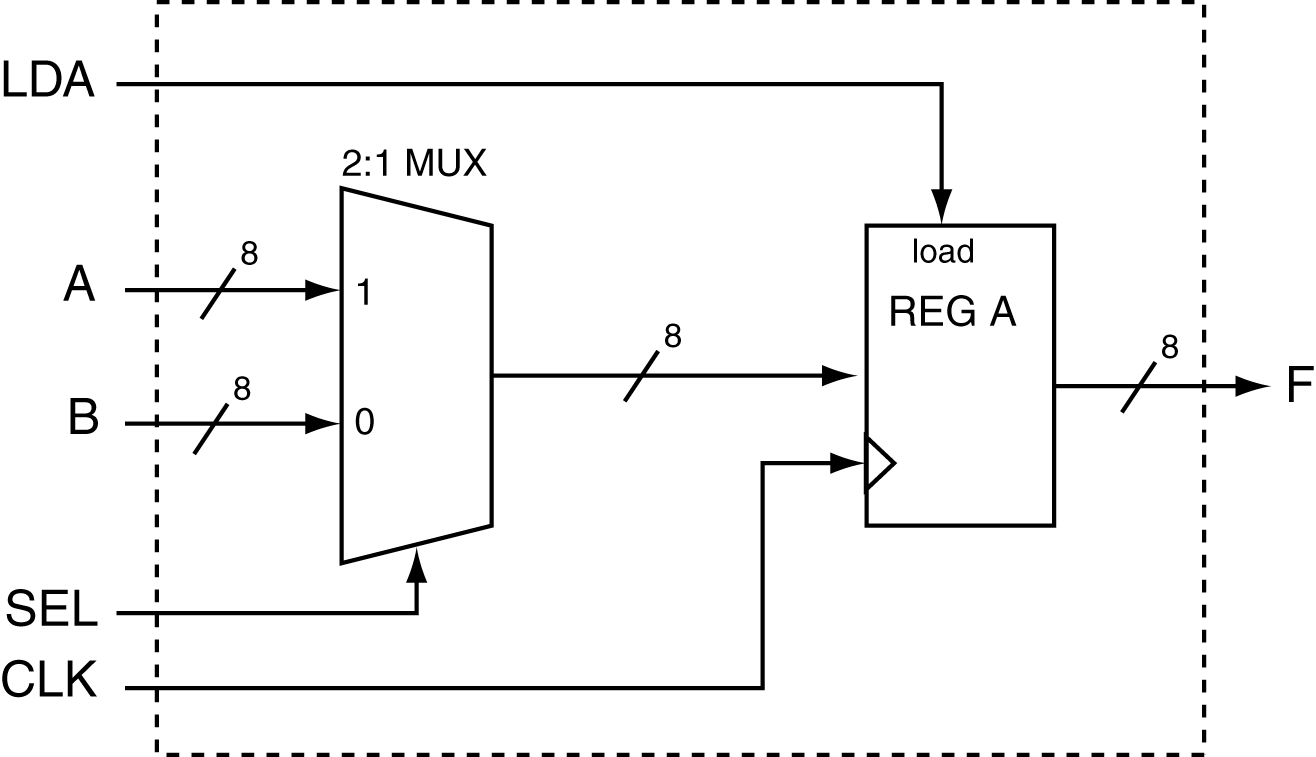
\includegraphics[width=6cm]{smu_vhdl/ex1.png}
\end{minipage}

%%%%%% EXERCISE 2 %%%%%%
\vspace{20pt}
\noindent
\begin{minipage}[t]{0.5\textwidth}
\textbf{EXERCISE 2.}
Provide a VHDL model that can be used to implement the following circuit.
\end{minipage}
\begin{minipage}[t]{0.47\textwidth}
\vspace{0pt}\raggedright
\centering
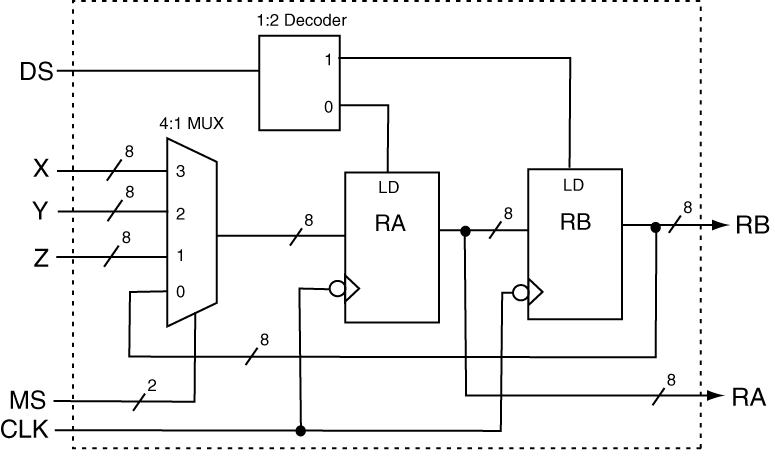
\includegraphics[width=6cm]{smu_vhdl/ex2.png}
\end{minipage}

%%%%%% EXERCISE 3 %%%%%%
\vspace{20pt}
\noindent
\begin{minipage}[t]{0.5\textwidth}
\textbf{EXERCISE 3.}
Provide a VHDL model that can be used to implement the following circuit. 
\end{minipage}
\begin{minipage}[t]{0.47\textwidth}
\vspace{0pt}\raggedright
\centering
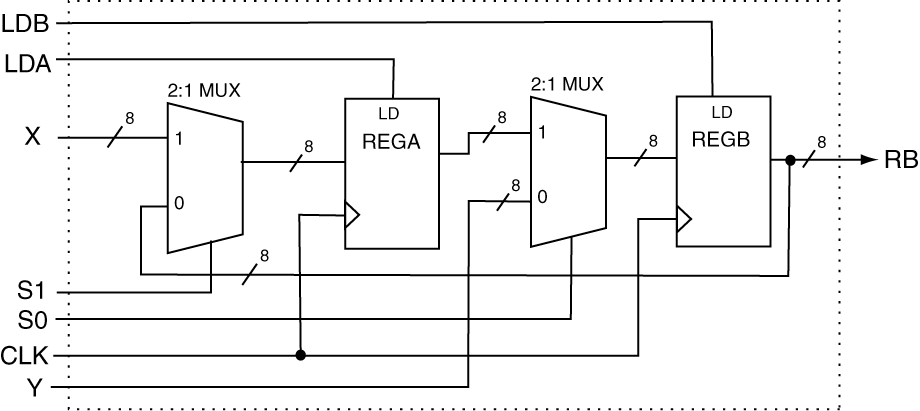
\includegraphics[width=6cm]{smu_vhdl/ex3.png}
\end{minipage}

%%%%%% EXERCISE 4 %%%%%%
\vspace{20pt}
\noindent
\begin{minipage}[t]{0.5\textwidth}
\textbf{EXERCISE 4.}
Provide a VHDL model that can be used to implement the following circuit.
\end{minipage}
\begin{minipage}[t]{0.47\textwidth}
\vspace{0pt}\raggedright
\centering
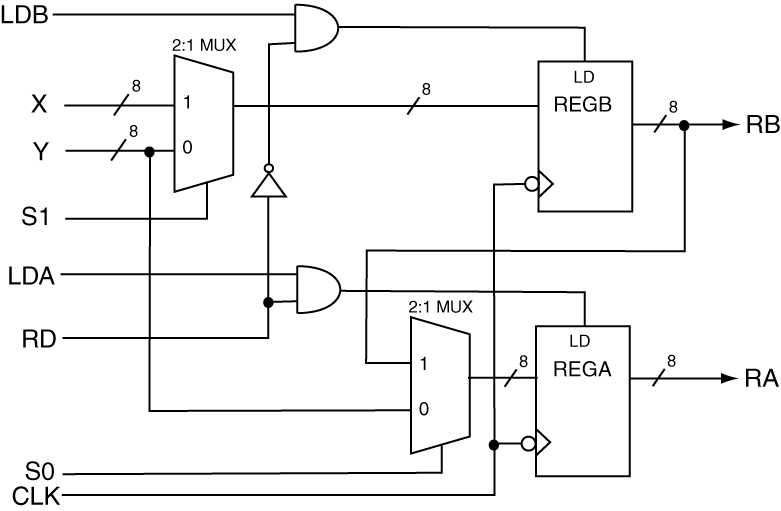
\includegraphics[width=6cm]{smu_vhdl/ex4.png}
\end{minipage}

%%%%%% EXERCISE 5 %%%%%%
\vspace{20pt}
\noindent
\begin{minipage}[t]{0.5\textwidth}
\textbf{EXERCISE 5.}
Provide a VHDL model that can be used to implement the following circuit.
\end{minipage}
\begin{minipage}[t]{0.47\textwidth}
\vspace{0pt}\raggedright
\centering
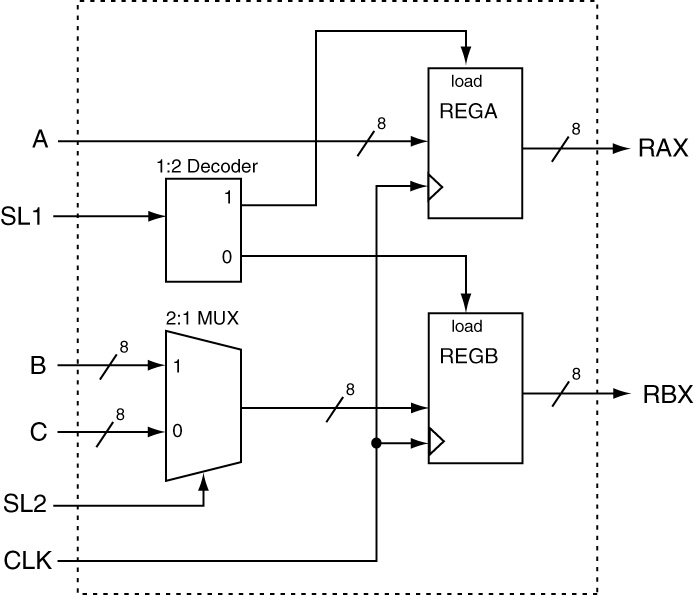
\includegraphics[width=6cm]{smu_vhdl/ex5.png}
\end{minipage}

%%%%%% EXERCISE 6 %%%%%%
\vspace{20pt}
\noindent
\begin{minipage}[t]{0.5\textwidth}
\textbf{EXERCISE 6.}
Provide a VHDL model that can be used to implement the following circuit.
\end{minipage}
\begin{minipage}[t]{0.47\textwidth}
\vspace{0pt}\raggedright
\centering
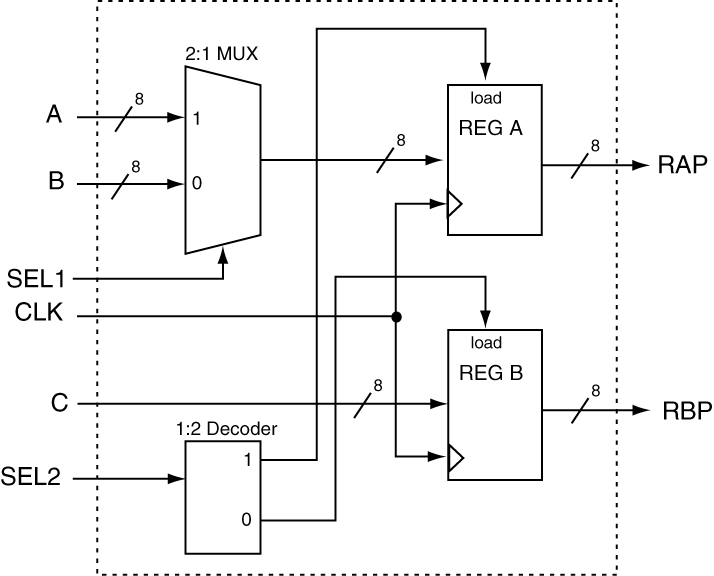
\includegraphics[width=6cm]{smu_vhdl/ex6.png}
\end{minipage}




